% Created by tikzDevice version 0.10.1 on 2016-08-14 10:49:32
% !TEX encoding = UTF-8 Unicode
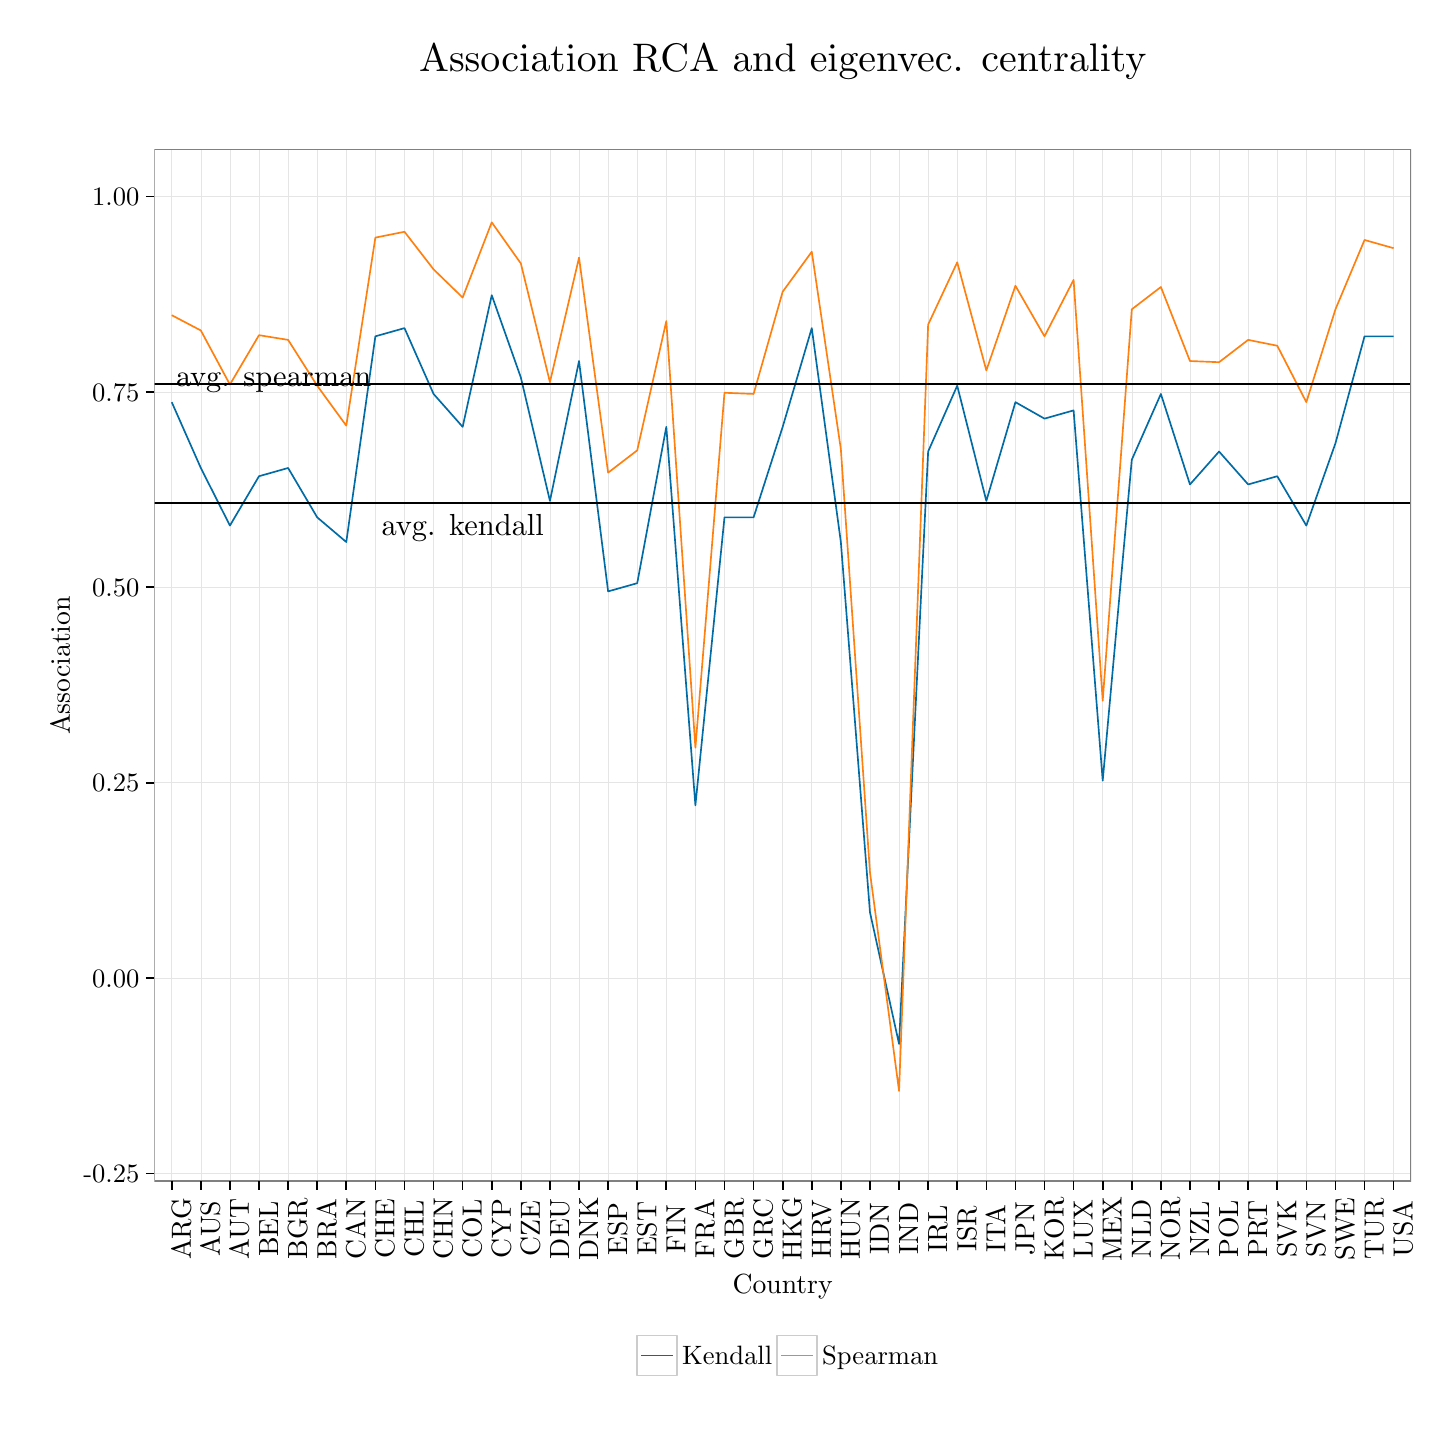
\begin{tikzpicture}[x=1pt,y=1pt]
\definecolor{fillColor}{RGB}{255,255,255}
\path[use as bounding box,fill=fillColor,fill opacity=0.00] (0,0) rectangle (505.89,505.89);
\begin{scope}
\path[clip] (  0.00,  0.00) rectangle (505.89,505.89);
\definecolor{drawColor}{RGB}{255,255,255}
\definecolor{fillColor}{RGB}{255,255,255}

\path[draw=drawColor,line width= 0.6pt,line join=round,line cap=round,fill=fillColor] (  0.00, -0.00) rectangle (505.89,505.89);
\end{scope}
\begin{scope}
\path[clip] ( 45.75, 89.02) rectangle (499.89,461.83);
\definecolor{fillColor}{RGB}{255,255,255}

\path[fill=fillColor] ( 45.75, 89.02) rectangle (499.89,461.83);
\definecolor{drawColor}{gray}{0.90}

\path[draw=drawColor,line width= 0.2pt,line join=round] ( 45.75, 91.84) --
	(499.89, 91.84);

\path[draw=drawColor,line width= 0.2pt,line join=round] ( 45.75,162.45) --
	(499.89,162.45);

\path[draw=drawColor,line width= 0.2pt,line join=round] ( 45.75,233.06) --
	(499.89,233.06);

\path[draw=drawColor,line width= 0.2pt,line join=round] ( 45.75,303.67) --
	(499.89,303.67);

\path[draw=drawColor,line width= 0.2pt,line join=round] ( 45.75,374.28) --
	(499.89,374.28);

\path[draw=drawColor,line width= 0.2pt,line join=round] ( 45.75,444.89) --
	(499.89,444.89);

\path[draw=drawColor,line width= 0.2pt,line join=round] ( 52.06, 89.02) --
	( 52.06,461.83);

\path[draw=drawColor,line width= 0.2pt,line join=round] ( 62.57, 89.02) --
	( 62.57,461.83);

\path[draw=drawColor,line width= 0.2pt,line join=round] ( 73.08, 89.02) --
	( 73.08,461.83);

\path[draw=drawColor,line width= 0.2pt,line join=round] ( 83.59, 89.02) --
	( 83.59,461.83);

\path[draw=drawColor,line width= 0.2pt,line join=round] ( 94.11, 89.02) --
	( 94.11,461.83);

\path[draw=drawColor,line width= 0.2pt,line join=round] (104.62, 89.02) --
	(104.62,461.83);

\path[draw=drawColor,line width= 0.2pt,line join=round] (115.13, 89.02) --
	(115.13,461.83);

\path[draw=drawColor,line width= 0.2pt,line join=round] (125.64, 89.02) --
	(125.64,461.83);

\path[draw=drawColor,line width= 0.2pt,line join=round] (136.16, 89.02) --
	(136.16,461.83);

\path[draw=drawColor,line width= 0.2pt,line join=round] (146.67, 89.02) --
	(146.67,461.83);

\path[draw=drawColor,line width= 0.2pt,line join=round] (157.18, 89.02) --
	(157.18,461.83);

\path[draw=drawColor,line width= 0.2pt,line join=round] (167.69, 89.02) --
	(167.69,461.83);

\path[draw=drawColor,line width= 0.2pt,line join=round] (178.21, 89.02) --
	(178.21,461.83);

\path[draw=drawColor,line width= 0.2pt,line join=round] (188.72, 89.02) --
	(188.72,461.83);

\path[draw=drawColor,line width= 0.2pt,line join=round] (199.23, 89.02) --
	(199.23,461.83);

\path[draw=drawColor,line width= 0.2pt,line join=round] (209.74, 89.02) --
	(209.74,461.83);

\path[draw=drawColor,line width= 0.2pt,line join=round] (220.26, 89.02) --
	(220.26,461.83);

\path[draw=drawColor,line width= 0.2pt,line join=round] (230.77, 89.02) --
	(230.77,461.83);

\path[draw=drawColor,line width= 0.2pt,line join=round] (241.28, 89.02) --
	(241.28,461.83);

\path[draw=drawColor,line width= 0.2pt,line join=round] (251.79, 89.02) --
	(251.79,461.83);

\path[draw=drawColor,line width= 0.2pt,line join=round] (262.31, 89.02) --
	(262.31,461.83);

\path[draw=drawColor,line width= 0.2pt,line join=round] (272.82, 89.02) --
	(272.82,461.83);

\path[draw=drawColor,line width= 0.2pt,line join=round] (283.33, 89.02) --
	(283.33,461.83);

\path[draw=drawColor,line width= 0.2pt,line join=round] (293.84, 89.02) --
	(293.84,461.83);

\path[draw=drawColor,line width= 0.2pt,line join=round] (304.36, 89.02) --
	(304.36,461.83);

\path[draw=drawColor,line width= 0.2pt,line join=round] (314.87, 89.02) --
	(314.87,461.83);

\path[draw=drawColor,line width= 0.2pt,line join=round] (325.38, 89.02) --
	(325.38,461.83);

\path[draw=drawColor,line width= 0.2pt,line join=round] (335.89, 89.02) --
	(335.89,461.83);

\path[draw=drawColor,line width= 0.2pt,line join=round] (346.41, 89.02) --
	(346.41,461.83);

\path[draw=drawColor,line width= 0.2pt,line join=round] (356.92, 89.02) --
	(356.92,461.83);

\path[draw=drawColor,line width= 0.2pt,line join=round] (367.43, 89.02) --
	(367.43,461.83);

\path[draw=drawColor,line width= 0.2pt,line join=round] (377.94, 89.02) --
	(377.94,461.83);

\path[draw=drawColor,line width= 0.2pt,line join=round] (388.46, 89.02) --
	(388.46,461.83);

\path[draw=drawColor,line width= 0.2pt,line join=round] (398.97, 89.02) --
	(398.97,461.83);

\path[draw=drawColor,line width= 0.2pt,line join=round] (409.48, 89.02) --
	(409.48,461.83);

\path[draw=drawColor,line width= 0.2pt,line join=round] (419.99, 89.02) --
	(419.99,461.83);

\path[draw=drawColor,line width= 0.2pt,line join=round] (430.51, 89.02) --
	(430.51,461.83);

\path[draw=drawColor,line width= 0.2pt,line join=round] (441.02, 89.02) --
	(441.02,461.83);

\path[draw=drawColor,line width= 0.2pt,line join=round] (451.53, 89.02) --
	(451.53,461.83);

\path[draw=drawColor,line width= 0.2pt,line join=round] (462.04, 89.02) --
	(462.04,461.83);

\path[draw=drawColor,line width= 0.2pt,line join=round] (472.56, 89.02) --
	(472.56,461.83);

\path[draw=drawColor,line width= 0.2pt,line join=round] (483.07, 89.02) --
	(483.07,461.83);

\path[draw=drawColor,line width= 0.2pt,line join=round] (493.58, 89.02) --
	(493.58,461.83);
\definecolor{drawColor}{RGB}{0,107,164}

\path[draw=drawColor,line width= 0.6pt,line join=round] ( 52.06,370.56) --
	( 62.57,346.78) --
	( 73.08,325.97) --
	( 83.59,343.80) --
	( 94.11,346.78) --
	(104.62,328.94) --
	(115.13,320.02) --
	(125.64,394.35) --
	(136.16,397.32) --
	(146.67,373.53) --
	(157.18,361.64) --
	(167.69,409.21) --
	(178.21,379.48) --
	(188.72,334.88) --
	(199.23,385.43) --
	(209.74,302.18) --
	(220.26,305.15) --
	(230.77,361.64) --
	(241.28,224.88) --
	(251.79,328.94) --
	(262.31,328.94) --
	(272.82,361.64) --
	(283.33,397.32) --
	(293.84,320.02) --
	(304.36,186.23) --
	(314.87,138.66) --
	(325.38,352.72) --
	(335.89,376.51) --
	(346.41,334.88) --
	(356.92,370.56) --
	(367.43,364.61) --
	(377.94,367.59) --
	(388.46,233.80) --
	(398.97,349.75) --
	(409.48,373.53) --
	(419.99,340.83) --
	(430.51,352.72) --
	(441.02,340.83) --
	(451.53,343.80) --
	(462.04,325.97) --
	(472.56,355.70) --
	(483.07,394.35) --
	(493.58,394.35);
\definecolor{drawColor}{RGB}{255,128,14}

\path[draw=drawColor,line width= 0.6pt,line join=round] ( 52.06,401.99) --
	( 62.57,396.47) --
	( 73.08,376.93) --
	( 83.59,394.77) --
	( 94.11,393.07) --
	(104.62,376.51) --
	(115.13,362.07) --
	(125.64,430.02) --
	(136.16,432.14) --
	(146.67,418.55) --
	(157.18,408.36) --
	(167.69,435.54) --
	(178.21,420.68) --
	(188.72,377.78) --
	(199.23,422.80) --
	(209.74,345.08) --
	(220.26,353.15) --
	(230.77,399.87) --
	(241.28,245.69) --
	(251.79,373.96) --
	(262.31,373.53) --
	(272.82,410.48) --
	(283.33,424.92) --
	(293.84,353.57) --
	(304.36,200.67) --
	(314.87,121.68) --
	(325.38,398.59) --
	(335.89,421.10) --
	(346.41,382.03) --
	(356.92,412.61) --
	(367.43,394.35) --
	(377.94,414.73) --
	(388.46,262.68) --
	(398.97,404.11) --
	(409.48,412.18) --
	(419.99,385.43) --
	(430.51,385.00) --
	(441.02,393.07) --
	(451.53,390.95) --
	(462.04,370.56) --
	(472.56,404.11) --
	(483.07,429.17) --
	(493.58,426.20);
\definecolor{drawColor}{RGB}{0,0,0}

\path[draw=drawColor,line width= 0.6pt,line join=round] ( 45.75,377.10) -- (499.89,377.10);

\node[text=drawColor,anchor=base,inner sep=0pt, outer sep=0pt, scale=  1.10] at ( 88.85,376.12) {avg. spearman};

\path[draw=drawColor,line width= 0.6pt,line join=round] ( 45.75,334.17) -- (499.89,334.17);

\node[text=drawColor,anchor=base,inner sep=0pt, outer sep=0pt, scale=  1.10] at (157.18,322.46) {avg. kendall};
\definecolor{drawColor}{gray}{0.50}

\path[draw=drawColor,line width= 0.6pt,line join=round,line cap=round] ( 45.75, 89.02) rectangle (499.89,461.83);
\end{scope}
\begin{scope}
\path[clip] (  0.00,  0.00) rectangle (505.89,505.89);
\definecolor{drawColor}{RGB}{0,0,0}

\node[text=drawColor,anchor=base east,inner sep=0pt, outer sep=0pt, scale=  0.96] at ( 40.35, 88.53) {-0.25};

\node[text=drawColor,anchor=base east,inner sep=0pt, outer sep=0pt, scale=  0.96] at ( 40.35,159.14) {0.00};

\node[text=drawColor,anchor=base east,inner sep=0pt, outer sep=0pt, scale=  0.96] at ( 40.35,229.75) {0.25};

\node[text=drawColor,anchor=base east,inner sep=0pt, outer sep=0pt, scale=  0.96] at ( 40.35,300.36) {0.50};

\node[text=drawColor,anchor=base east,inner sep=0pt, outer sep=0pt, scale=  0.96] at ( 40.35,370.97) {0.75};

\node[text=drawColor,anchor=base east,inner sep=0pt, outer sep=0pt, scale=  0.96] at ( 40.35,441.58) {1.00};
\end{scope}
\begin{scope}
\path[clip] (  0.00,  0.00) rectangle (505.89,505.89);
\definecolor{drawColor}{RGB}{0,0,0}

\path[draw=drawColor,line width= 0.6pt,line join=round] ( 42.75, 91.84) --
	( 45.75, 91.84);

\path[draw=drawColor,line width= 0.6pt,line join=round] ( 42.75,162.45) --
	( 45.75,162.45);

\path[draw=drawColor,line width= 0.6pt,line join=round] ( 42.75,233.06) --
	( 45.75,233.06);

\path[draw=drawColor,line width= 0.6pt,line join=round] ( 42.75,303.67) --
	( 45.75,303.67);

\path[draw=drawColor,line width= 0.6pt,line join=round] ( 42.75,374.28) --
	( 45.75,374.28);

\path[draw=drawColor,line width= 0.6pt,line join=round] ( 42.75,444.89) --
	( 45.75,444.89);
\end{scope}
\begin{scope}
\path[clip] (  0.00,  0.00) rectangle (505.89,505.89);
\definecolor{drawColor}{RGB}{0,0,0}

\path[draw=drawColor,line width= 0.6pt,line join=round] ( 52.06, 86.02) --
	( 52.06, 89.02);

\path[draw=drawColor,line width= 0.6pt,line join=round] ( 62.57, 86.02) --
	( 62.57, 89.02);

\path[draw=drawColor,line width= 0.6pt,line join=round] ( 73.08, 86.02) --
	( 73.08, 89.02);

\path[draw=drawColor,line width= 0.6pt,line join=round] ( 83.59, 86.02) --
	( 83.59, 89.02);

\path[draw=drawColor,line width= 0.6pt,line join=round] ( 94.11, 86.02) --
	( 94.11, 89.02);

\path[draw=drawColor,line width= 0.6pt,line join=round] (104.62, 86.02) --
	(104.62, 89.02);

\path[draw=drawColor,line width= 0.6pt,line join=round] (115.13, 86.02) --
	(115.13, 89.02);

\path[draw=drawColor,line width= 0.6pt,line join=round] (125.64, 86.02) --
	(125.64, 89.02);

\path[draw=drawColor,line width= 0.6pt,line join=round] (136.16, 86.02) --
	(136.16, 89.02);

\path[draw=drawColor,line width= 0.6pt,line join=round] (146.67, 86.02) --
	(146.67, 89.02);

\path[draw=drawColor,line width= 0.6pt,line join=round] (157.18, 86.02) --
	(157.18, 89.02);

\path[draw=drawColor,line width= 0.6pt,line join=round] (167.69, 86.02) --
	(167.69, 89.02);

\path[draw=drawColor,line width= 0.6pt,line join=round] (178.21, 86.02) --
	(178.21, 89.02);

\path[draw=drawColor,line width= 0.6pt,line join=round] (188.72, 86.02) --
	(188.72, 89.02);

\path[draw=drawColor,line width= 0.6pt,line join=round] (199.23, 86.02) --
	(199.23, 89.02);

\path[draw=drawColor,line width= 0.6pt,line join=round] (209.74, 86.02) --
	(209.74, 89.02);

\path[draw=drawColor,line width= 0.6pt,line join=round] (220.26, 86.02) --
	(220.26, 89.02);

\path[draw=drawColor,line width= 0.6pt,line join=round] (230.77, 86.02) --
	(230.77, 89.02);

\path[draw=drawColor,line width= 0.6pt,line join=round] (241.28, 86.02) --
	(241.28, 89.02);

\path[draw=drawColor,line width= 0.6pt,line join=round] (251.79, 86.02) --
	(251.79, 89.02);

\path[draw=drawColor,line width= 0.6pt,line join=round] (262.31, 86.02) --
	(262.31, 89.02);

\path[draw=drawColor,line width= 0.6pt,line join=round] (272.82, 86.02) --
	(272.82, 89.02);

\path[draw=drawColor,line width= 0.6pt,line join=round] (283.33, 86.02) --
	(283.33, 89.02);

\path[draw=drawColor,line width= 0.6pt,line join=round] (293.84, 86.02) --
	(293.84, 89.02);

\path[draw=drawColor,line width= 0.6pt,line join=round] (304.36, 86.02) --
	(304.36, 89.02);

\path[draw=drawColor,line width= 0.6pt,line join=round] (314.87, 86.02) --
	(314.87, 89.02);

\path[draw=drawColor,line width= 0.6pt,line join=round] (325.38, 86.02) --
	(325.38, 89.02);

\path[draw=drawColor,line width= 0.6pt,line join=round] (335.89, 86.02) --
	(335.89, 89.02);

\path[draw=drawColor,line width= 0.6pt,line join=round] (346.41, 86.02) --
	(346.41, 89.02);

\path[draw=drawColor,line width= 0.6pt,line join=round] (356.92, 86.02) --
	(356.92, 89.02);

\path[draw=drawColor,line width= 0.6pt,line join=round] (367.43, 86.02) --
	(367.43, 89.02);

\path[draw=drawColor,line width= 0.6pt,line join=round] (377.94, 86.02) --
	(377.94, 89.02);

\path[draw=drawColor,line width= 0.6pt,line join=round] (388.46, 86.02) --
	(388.46, 89.02);

\path[draw=drawColor,line width= 0.6pt,line join=round] (398.97, 86.02) --
	(398.97, 89.02);

\path[draw=drawColor,line width= 0.6pt,line join=round] (409.48, 86.02) --
	(409.48, 89.02);

\path[draw=drawColor,line width= 0.6pt,line join=round] (419.99, 86.02) --
	(419.99, 89.02);

\path[draw=drawColor,line width= 0.6pt,line join=round] (430.51, 86.02) --
	(430.51, 89.02);

\path[draw=drawColor,line width= 0.6pt,line join=round] (441.02, 86.02) --
	(441.02, 89.02);

\path[draw=drawColor,line width= 0.6pt,line join=round] (451.53, 86.02) --
	(451.53, 89.02);

\path[draw=drawColor,line width= 0.6pt,line join=round] (462.04, 86.02) --
	(462.04, 89.02);

\path[draw=drawColor,line width= 0.6pt,line join=round] (472.56, 86.02) --
	(472.56, 89.02);

\path[draw=drawColor,line width= 0.6pt,line join=round] (483.07, 86.02) --
	(483.07, 89.02);

\path[draw=drawColor,line width= 0.6pt,line join=round] (493.58, 86.02) --
	(493.58, 89.02);
\end{scope}
\begin{scope}
\path[clip] (  0.00,  0.00) rectangle (505.89,505.89);
\definecolor{drawColor}{RGB}{0,0,0}

\node[text=drawColor,rotate= 90.00,anchor=base,inner sep=0pt, outer sep=0pt, scale=  1.00] at ( 58.94, 71.88) {ARG};

\node[text=drawColor,rotate= 90.00,anchor=base,inner sep=0pt, outer sep=0pt, scale=  1.00] at ( 69.46, 71.88) {AUS};

\node[text=drawColor,rotate= 90.00,anchor=base,inner sep=0pt, outer sep=0pt, scale=  1.00] at ( 79.97, 71.88) {AUT};

\node[text=drawColor,rotate= 90.00,anchor=base,inner sep=0pt, outer sep=0pt, scale=  1.00] at ( 90.48, 71.88) {BEL};

\node[text=drawColor,rotate= 90.00,anchor=base,inner sep=0pt, outer sep=0pt, scale=  1.00] at (100.99, 71.88) {BGR};

\node[text=drawColor,rotate= 90.00,anchor=base,inner sep=0pt, outer sep=0pt, scale=  1.00] at (111.51, 71.88) {BRA};

\node[text=drawColor,rotate= 90.00,anchor=base,inner sep=0pt, outer sep=0pt, scale=  1.00] at (122.02, 71.88) {CAN};

\node[text=drawColor,rotate= 90.00,anchor=base,inner sep=0pt, outer sep=0pt, scale=  1.00] at (132.53, 71.88) {CHE};

\node[text=drawColor,rotate= 90.00,anchor=base,inner sep=0pt, outer sep=0pt, scale=  1.00] at (143.04, 71.88) {CHL};

\node[text=drawColor,rotate= 90.00,anchor=base,inner sep=0pt, outer sep=0pt, scale=  1.00] at (153.56, 71.88) {CHN};

\node[text=drawColor,rotate= 90.00,anchor=base,inner sep=0pt, outer sep=0pt, scale=  1.00] at (164.07, 71.88) {COL};

\node[text=drawColor,rotate= 90.00,anchor=base,inner sep=0pt, outer sep=0pt, scale=  1.00] at (174.58, 71.88) {CYP};

\node[text=drawColor,rotate= 90.00,anchor=base,inner sep=0pt, outer sep=0pt, scale=  1.00] at (185.09, 71.88) {CZE};

\node[text=drawColor,rotate= 90.00,anchor=base,inner sep=0pt, outer sep=0pt, scale=  1.00] at (195.61, 71.88) {DEU};

\node[text=drawColor,rotate= 90.00,anchor=base,inner sep=0pt, outer sep=0pt, scale=  1.00] at (206.12, 71.88) {DNK};

\node[text=drawColor,rotate= 90.00,anchor=base,inner sep=0pt, outer sep=0pt, scale=  1.00] at (216.63, 71.88) {ESP};

\node[text=drawColor,rotate= 90.00,anchor=base,inner sep=0pt, outer sep=0pt, scale=  1.00] at (227.14, 71.88) {EST};

\node[text=drawColor,rotate= 90.00,anchor=base,inner sep=0pt, outer sep=0pt, scale=  1.00] at (237.66, 71.88) {FIN};

\node[text=drawColor,rotate= 90.00,anchor=base,inner sep=0pt, outer sep=0pt, scale=  1.00] at (248.17, 71.88) {FRA};

\node[text=drawColor,rotate= 90.00,anchor=base,inner sep=0pt, outer sep=0pt, scale=  1.00] at (258.68, 71.88) {GBR};

\node[text=drawColor,rotate= 90.00,anchor=base,inner sep=0pt, outer sep=0pt, scale=  1.00] at (269.19, 71.88) {GRC};

\node[text=drawColor,rotate= 90.00,anchor=base,inner sep=0pt, outer sep=0pt, scale=  1.00] at (279.71, 71.88) {HKG};

\node[text=drawColor,rotate= 90.00,anchor=base,inner sep=0pt, outer sep=0pt, scale=  1.00] at (290.22, 71.88) {HRV};

\node[text=drawColor,rotate= 90.00,anchor=base,inner sep=0pt, outer sep=0pt, scale=  1.00] at (300.73, 71.88) {HUN};

\node[text=drawColor,rotate= 90.00,anchor=base,inner sep=0pt, outer sep=0pt, scale=  1.00] at (311.24, 71.88) {IDN};

\node[text=drawColor,rotate= 90.00,anchor=base,inner sep=0pt, outer sep=0pt, scale=  1.00] at (321.76, 71.88) {IND};

\node[text=drawColor,rotate= 90.00,anchor=base,inner sep=0pt, outer sep=0pt, scale=  1.00] at (332.27, 71.88) {IRL};

\node[text=drawColor,rotate= 90.00,anchor=base,inner sep=0pt, outer sep=0pt, scale=  1.00] at (342.78, 71.88) {ISR};

\node[text=drawColor,rotate= 90.00,anchor=base,inner sep=0pt, outer sep=0pt, scale=  1.00] at (353.29, 71.88) {ITA};

\node[text=drawColor,rotate= 90.00,anchor=base,inner sep=0pt, outer sep=0pt, scale=  1.00] at (363.81, 71.88) {JPN};

\node[text=drawColor,rotate= 90.00,anchor=base,inner sep=0pt, outer sep=0pt, scale=  1.00] at (374.32, 71.88) {KOR};

\node[text=drawColor,rotate= 90.00,anchor=base,inner sep=0pt, outer sep=0pt, scale=  1.00] at (384.83, 71.88) {LUX};

\node[text=drawColor,rotate= 90.00,anchor=base,inner sep=0pt, outer sep=0pt, scale=  1.00] at (395.34, 71.88) {MEX};

\node[text=drawColor,rotate= 90.00,anchor=base,inner sep=0pt, outer sep=0pt, scale=  1.00] at (405.86, 71.88) {NLD};

\node[text=drawColor,rotate= 90.00,anchor=base,inner sep=0pt, outer sep=0pt, scale=  1.00] at (416.37, 71.88) {NOR};

\node[text=drawColor,rotate= 90.00,anchor=base,inner sep=0pt, outer sep=0pt, scale=  1.00] at (426.88, 71.88) {NZL};

\node[text=drawColor,rotate= 90.00,anchor=base,inner sep=0pt, outer sep=0pt, scale=  1.00] at (437.39, 71.88) {POL};

\node[text=drawColor,rotate= 90.00,anchor=base,inner sep=0pt, outer sep=0pt, scale=  1.00] at (447.91, 71.88) {PRT};

\node[text=drawColor,rotate= 90.00,anchor=base,inner sep=0pt, outer sep=0pt, scale=  1.00] at (458.42, 71.88) {SVK};

\node[text=drawColor,rotate= 90.00,anchor=base,inner sep=0pt, outer sep=0pt, scale=  1.00] at (468.93, 71.88) {SVN};

\node[text=drawColor,rotate= 90.00,anchor=base,inner sep=0pt, outer sep=0pt, scale=  1.00] at (479.44, 71.88) {SWE};

\node[text=drawColor,rotate= 90.00,anchor=base,inner sep=0pt, outer sep=0pt, scale=  1.00] at (489.96, 71.88) {TUR};

\node[text=drawColor,rotate= 90.00,anchor=base,inner sep=0pt, outer sep=0pt, scale=  1.00] at (500.47, 71.88) {USA};
\end{scope}
\begin{scope}
\path[clip] (  0.00,  0.00) rectangle (505.89,505.89);
\definecolor{drawColor}{RGB}{0,0,0}

\node[text=drawColor,anchor=base,inner sep=0pt, outer sep=0pt, scale=  1.00] at (272.82, 48.46) {Country};
\end{scope}
\begin{scope}
\path[clip] (  0.00,  0.00) rectangle (505.89,505.89);
\definecolor{drawColor}{RGB}{0,0,0}

\node[text=drawColor,rotate= 90.00,anchor=base,inner sep=0pt, outer sep=0pt, scale=  1.00] at ( 15.29,275.42) {Association};
\end{scope}
\begin{scope}
\path[clip] (  0.00,  0.00) rectangle (505.89,505.89);
\definecolor{fillColor}{RGB}{255,255,255}

\path[fill=fillColor] (212.38, 14.54) rectangle (333.26, 37.53);
\end{scope}
\begin{scope}
\path[clip] (  0.00,  0.00) rectangle (505.89,505.89);
\definecolor{drawColor}{gray}{0.80}
\definecolor{fillColor}{RGB}{255,255,255}

\path[draw=drawColor,line width= 0.6pt,line join=round,line cap=round,fill=fillColor] (220.26, 18.80) rectangle (234.71, 33.26);
\end{scope}
\begin{scope}
\path[clip] (  0.00,  0.00) rectangle (505.89,505.89);
\definecolor{drawColor}{RGB}{0,107,164}

\path[draw=drawColor,line width= 0.6pt,line join=round] (221.70, 26.03) -- (233.27, 26.03);
\end{scope}
\begin{scope}
\path[clip] (  0.00,  0.00) rectangle (505.89,505.89);
\definecolor{drawColor}{gray}{0.80}
\definecolor{fillColor}{RGB}{255,255,255}

\path[draw=drawColor,line width= 0.6pt,line join=round,line cap=round,fill=fillColor] (270.85, 18.80) rectangle (285.30, 33.26);
\end{scope}
\begin{scope}
\path[clip] (  0.00,  0.00) rectangle (505.89,505.89);
\definecolor{drawColor}{RGB}{255,128,14}

\path[draw=drawColor,line width= 0.6pt,line join=round] (272.30, 26.03) -- (283.86, 26.03);
\end{scope}
\begin{scope}
\path[clip] (  0.00,  0.00) rectangle (505.89,505.89);
\definecolor{drawColor}{RGB}{0,0,0}

\node[text=drawColor,anchor=base west,inner sep=0pt, outer sep=0pt, scale=  0.96] at (236.52, 22.72) {Kendall};
\end{scope}
\begin{scope}
\path[clip] (  0.00,  0.00) rectangle (505.89,505.89);
\definecolor{drawColor}{RGB}{0,0,0}

\node[text=drawColor,anchor=base west,inner sep=0pt, outer sep=0pt, scale=  0.96] at (287.11, 22.72) {Spearman};
\end{scope}
\begin{scope}
\path[clip] (  0.00,  0.00) rectangle (505.89,505.89);
\definecolor{drawColor}{RGB}{0,0,0}

\node[text=drawColor,anchor=base west,inner sep=0pt, outer sep=0pt, scale=  1.44] at (141.45,489.97) {Association RCA and eigenvec. centrality};
\end{scope}
\end{tikzpicture}
